%----------------------------------------------------------------------------------------
%	PACKAGES AND DOCUMENT CONFIGURATIONS
%----------------------------------------------------------------------------------------

\documentclass{article}

\usepackage{graphicx} % Required for the inclusion of images

\usepackage[utf8]{inputenc}

\usepackage[justification=centering]{caption}
\usepackage{caption}
\usepackage{subcaption}
\usepackage{amsmath,amssymb,amsfonts,amsthm,mathtools}
\usepackage{xfrac}
\usepackage{float}

\usepackage{hyperref}
\usepackage{url}
\usepackage{array}
\usepackage[flushleft]{threeparttable}

\usepackage{comment}
\usepackage[font=small,labelfont=bf]{caption}


\usepackage{listings, lstautogobble}
\usepackage{fancyhdr}
\usepackage{graphicx}
\usepackage{hyperref}

\graphicspath{ {./} }
\setlength\parskip{4pt}
\setlength\parindent{0pt}
\setlength{\tabcolsep}{8pt}
\renewcommand{\arraystretch}{1.5}
% \setlength{\tabcolsep}{8pt}
% \renewcommand{\arraystretch}{1.5}

%\usepackage{times} % Uncomment to use the Times New Roman font

%----------------------------------------------------------------------------------------
%	DOCUMENT INFORMATION
%----------------------------------------------------------------------------------------

\title
{
	\LARGE\textbf{Dog detection} \\ 
	Neural network course project \\
	\author
	{ 
		Jakub \textsc{Zadrożny}, 
		Mateusz \textsc{Hazy},
		Kamil \textsc{Szubiński}
	}
}
\date{\today}

\begin{document}
\maketitle

\section*{Abstract}

Object detection is a very rapidly evolving deep learning area and a wide variety of methods has been developed in recent years. Many of them suffer from a computation complexity (RCNN). In this paper we revisit YOLO \cite{yolo} and YOLO 9000 \cite{yolo9000} - fast real time object detection methods. Both of them are able to detect many classes of objects, however, we limit ourselves to detecting only one class - a dog. We then compare our results with the original ones and with other methods such as RCNN and Fast RCNN.

\section*{YOLO}

The YOLO method states detection as a linear regression problem straight from pixels to bounding boxes coordinates and class probabilities. The system divides image into $ S \times S $ grid. If the center of an object falls into a grid cell, that grid cell is responsible for detecting that object. Each grid cell can predict $B$ bounding boxes. Each bounding box consists of five predictions: $x, y, w, h$ and confidence, where the first four describe the bounding box location and size. The last parameter describes how confident the model is that the bounding box contains the object. Overall the YOLO architecture takes the image, passes it through convolutional and fully connected layers and produces $S \times S \times (B \cdot  5 + C)$ predictions. Each $B \cdot 5 + C$ segment represents the predictions for the grid cell. Five parameters described above for each bounding box and C class probabilities. The original paper \cite{yolo} provides more detailed description.
\section*{YOLO 9000}

TODO 

\section*{Dataset}
We decided to use a subset of Youtube-BoundingBoxes Dataset \cite{youtube-bb}. One can find there more than 200000 frames with dogs. The biggest disadvantage of this dataset is that only one object is detected in every frame. This can lead to some troubles with learning the model. The other problem is that some bounding boxes are set incorrectly. However, this can reduce overfitting during learning.

\begin{figure}[H]

\begin{minipage}{.4\textwidth}
	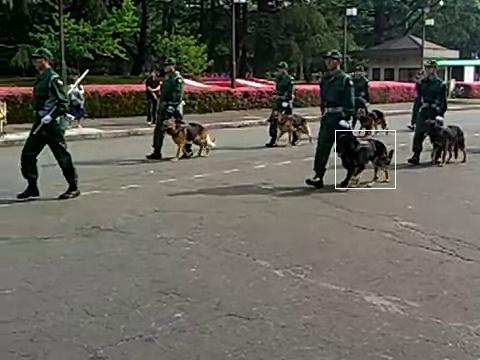
\includegraphics[width=\textwidth]{multiple_dogs.jpg}
	\caption{Image with many dogs, where only one is detected.}
\end{minipage}%
\hfill
\begin{minipage}{.4\textwidth}
	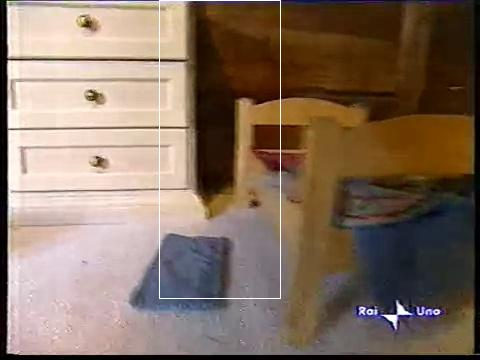
\includegraphics[width=\textwidth]{wrong_bb.jpg}
	\caption{Image with wrong bounding box.}
\end{minipage}%
\hfill

\end{figure}


\section*{Training}

We took 8000 of the images of dogs from Youtube-BoundingBoxes Dataset and did traiditional train/test split. Then we used Adam as an optimizer. \\

We optimized the weighted mean least squares error, as suggested in the paper \cite{yolo} \\

The error function was defined as:
$$ 1 - IOU(predicted\_box, true\_box)$$
where
$$ IOU(A, B) = \frac{ A \cap B}{A \cup B} $$

\subsection*{YOLO training}
As a feature extractor we tried to use pretrained vgg and resnet50 networks. On top of that we added 2 fully connected layers and ReLU for nonlinearity. For regularization we used drouput with $p = 0.5$. 

\begin{figure}[H]
	\begin{center}
		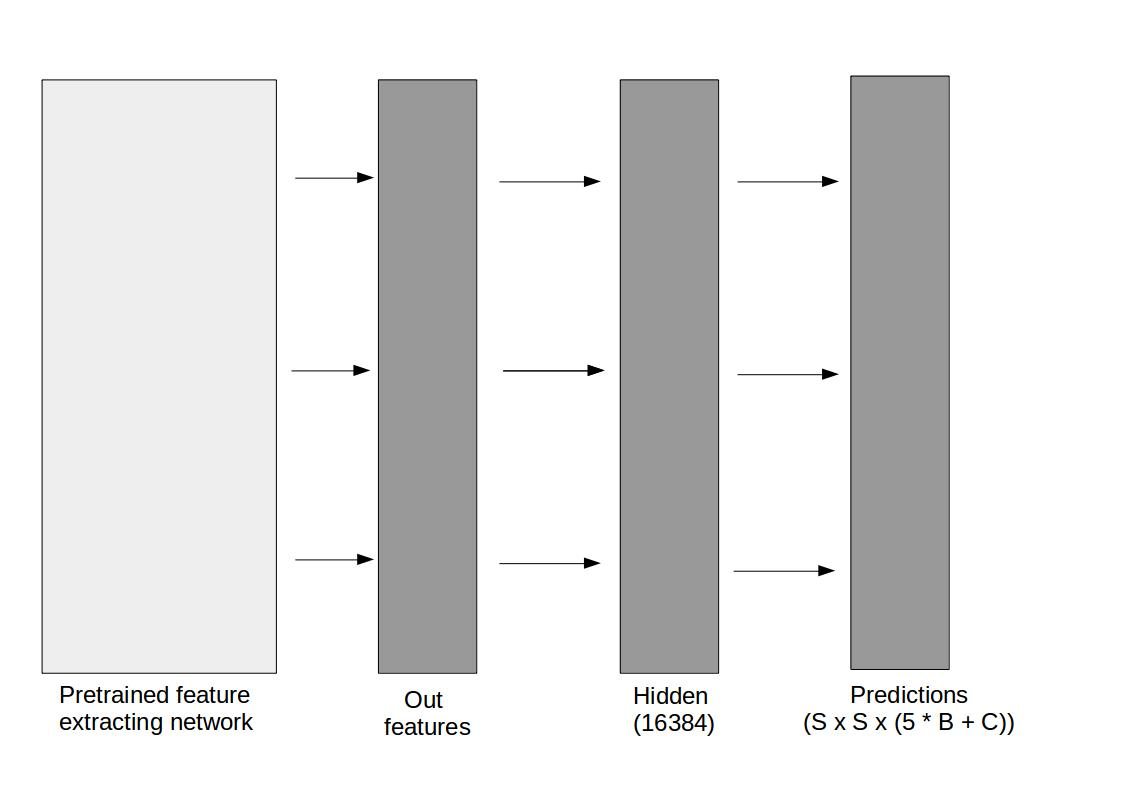
\includegraphics[width=10cm]{yolo_arch.jpg}\\
		\centering
		\caption{YOLO architecture}
	\end{center}
\hfill

\end{figure}

We managed to train the network down to 25\% train error rate. However the test error rate has never been smaller than 65\%. We tried different configurations of hyperparameters, adding noise to input values and data augmentation, yet it did not improve the results. We decided to abandon the YOLO approach and move to the YOLO 9000.

\subsection*{YOLO 9000}

\section*{Comparison with other methods}


\section*{Conclusion}




\newpage
\begin{thebibliography}{9}

\bibitem{yolo}
Joseph Redmon, Santosh Divvala, Ross Girshick, Ali Farhadi:
\\You Only Look Once: Unified, Real-Time Object Detection
\\\texttt{https://arxiv.org/pdf/1506.02640v5.pdf}

\bibitem{yolo9000}
Joseph Redmon, Ali Farhadi: YOLO9000:Better, Faster, Stronger
\\\texttt{https://arxiv.org/pdf/1612.08242v1.pdf}

\bibitem{youtube-bb}
\texttt{ https://research.google.com/youtube-bb/}

\end{thebibliography}

\end{document}